\documentclass[conference]{IEEEtran}
\IEEEoverridecommandlockouts
% The preceding line is only needed to identify funding in the first footnote. If that is unneeded, please comment it out.
\usepackage{cite}
\usepackage{amsmath,amssymb,amsfonts}
\usepackage{algorithmic}
\usepackage{graphicx}
\usepackage{textcomp}
\usepackage{xcolor}


\def\BibTeX{{\rm B\kern-.05em{\sc i\kern-.025em b}\kern-.08em
    T\kern-.1667em\lower.7ex\hbox{E}\kern-.125emX}}
\begin{document}

\title{MUSIC: Make Unification Simple In Image Classification \\}

\author{
    \IEEEauthorblockN{Muhammad Shahbaz\IEEEauthorrefmark{1}, 
                      Hamza Waheed\IEEEauthorrefmark{1}, 
                      Abdullah Asghar\IEEEauthorrefmark{1}, 
                      Abdul Wahab\IEEEauthorrefmark{1}}
    \IEEEauthorblockA{
        \textit{Masters in Data Science} \\
        \textit{FAST National University of Computer and Emerging Sciences} \\
        Emails: i248029@isb.nu.edu.pk, i247628@isb.nu.edu.pk, 
        i248000@isb.nu.edu.pk, wahab24@example.com
    }
}



\maketitle

\begin{abstract}
Training a model is the backbone of Machine learning because all the decisions will be done on its basis. Once it is trained we further improve it on the basis of feedback and our requirements. To perform this we use the process of fine-tuning, it is process to further retrain the pre-trained model on small target dataset, we combine multiple tasks and then retrain it on already trained model to improve the performance on these specific tasks. The accuracy achieved is very low after fine-tuning.We observed the flaw in the process that when we merge our tasks and then do fine-tuning, our performance decreases. To solve this issue the concept of MUSIC (Make Utility Simple In Image Classification) takes place, we simply fine-tune the model on each task individually instead of merging them as one and as a result we achieved accuracy of 88\% from 70\% which is a drastic difference. 
\end{abstract}

\begin{IEEEkeywords}
\vspace{0.5cm} \\ Fine-tuning, Editng models, Artificial Intelligence
\end{IEEEkeywords}

\section{Introduction}
In the last few years AI (Artificial Intelligence) has taken the world. AI models are trained on data to perform specific tasks. Common type of AI models include Supervised learning models which are trained in labeled data to predict outcomes such as regression and classification , Unsupervised learning models  which are trained on unlabeled data to identify patterns such as K means classification, Deep learning models which uses neural networks like humans and process complex data like images, voice notes etc. Models are used commonly as core of AI, we often edit them after training to achieve desired results. We train them to change the behavior, if we want to increase the response of specific class in case of classification then we need to retrain the model accordingly and vice versa. This process is called fine-tuning and it is different from training a model. In the context of training the model has not learned anything we assign it parameters and weights to operate while fine-tuning is process after training model where we take the pre trained model’s behavior as a starting point and then tune it on specific tasks. 

While performing fine tuning for experimentation on MNIST dataset we observed that overall our accuracy is decreasing, before fine tuning our accuracy was 91.70\% and after fine tuning our accuracy decreased to 70\% which is a huge difference. The proces of fine-tuning is very expensive as we need to follow the same steps which we follow while training the model first time so our time is utilized, resources are utilized as we need the current model and its parameters for fine-tuning, increase in the utilization of resources direcly impacts the cost due to which cost also increases. To smooth this process of retraining model new method was proposed which was editing models with task aritmmetic operations\cite{paper-1}. Here we use task vector which is basically our target to retrain the model , we use the arithmetic operation like subtraction or addition to retrain the pre-trained model.When we need to increase the reponse of a specific task we will make its vector and directly perform the addition of pretrained model and our task vector which results in new model which is now trained on new parameters according to your requirements and here the cost and resources used are very less as compared to fine-tuning , same is the cases with subtraction, if we want to decraese the response of task on model we will retrain it on that task. Task vectors are formed by the difference of fine-tuned model and pretrained model. It can be single task or combination of multiple tasks. Currently we will focus on the process of fine-tuning that how can we improve its accuracy and smoothens it. After that we will come to task arithmetic operations which is much better than fine-tuning in terms of cost and resources. 

\subsection*{Summary of the Fine-Tuning Process}
In this approach, the pre-trained model \( \mathcal{M} \) is fine-tuned incrementally on datasets corresponding to individual classes. Instead of merging datasets, we fine-tune the model sequentially for better class-specific learning.

\begin{enumerate}
    \item We begin by fine-tuning the pre-trained model on data from class 1, updating its parameters to \( \theta_1 \).
    \item Next, the model fine-tuned on class 1 is further fine-tuned on data from class 2, resulting in updated parameters \( \theta_2 \).
    \item Finally, the model fine-tuned on class 2 is fine-tuned on class 3, producing the final model with parameters \( \theta_3 \).
\end{enumerate}

This method ensures that each class contributes to the model's performance individually, preventing performance degradation that can arise from merging tasks. As a result, we achieved a significant accuracy improvement compared to merging all classes before fine-tuning.so we can say that best practice is to train model on each task individually instead of merging them and then training them.

\subsection{Methamatical Equations}
The fine-tuning process can be mathematically represented as follows:

1. Start with the pre-trained model:
\begin{equation}
\mathcal{M}_0(\theta_0)
\end{equation}

2. Fine-tune on the dataset of class 1 (\( \mathcal{D}_1 \)):
\begin{equation}
\mathcal{M}_1(\theta_1) = \arg \min_{\theta} \mathcal{L}(\mathcal{M}(\theta), \mathcal{D}_1)
\end{equation}

3. Fine-tune the updated model on the dataset of class 2 (\( \mathcal{D}_2 \)):
\begin{equation}
\mathcal{M}_2(\theta_2) = \arg \min_{\theta} \mathcal{L}(\mathcal{M}_1(\theta), \mathcal{D}_2)
\end{equation}

4. Fine-tune the updated model further on the dataset of class 3 (\( \mathcal{D}_3 \)):
\begin{equation}
\mathcal{M}_3(\theta_3) = \arg \min_{\theta} \mathcal{L}(\mathcal{M}_2(\theta), \mathcal{D}_3)
\end{equation}

Here:
\begin{itemize}
    \item \( \mathcal{L} \) represents the loss function (e.g., cross-entropy loss).
    \item \( \mathcal{M}_i(\theta_i) \) denotes the model fine-tuned after training on class \( i \).
\end{itemize}



\section{Related Work}
\paragraph{Editing Models with Task Arithmetic} Training a model is the backbone of Machine learning because all the decisions will be done on its basis\cite{paper-1}. Once training is done we retrain it according to our needs and feedback. This process is very costly due to following factors:
Time and capital is effected most on retraining as we need to perform that process again so more time is utilized due to which more money is exhausted. We only have trained model instead of training data so we need to collect it again so need resources to do it.
Fine tuning was introduced to address this problem but it requires labeled data so we need more efficient solution, here comes the solution of editing models with task arithmetic operations using task vectors. Task vector is weights in direction (Positive / Negative) which help the model to perform better.
For example if we want to mitigate undesirable behaviors then we can change behaviors of model by negating as task vector similarly if we can to make model to learn new thing then we can do it by adding task vector. This performs well target tasks or even also improves performance and also efficient to compute as compared to fine tuning.

\paragraph{LANGUAGE MODELS ARE HOMER SIMPSON! Safety Re-Alignment of Fine-tuned Language Models through Task Arithmetic} The introduction tells about the advances and growth of LLMs\cite{paper-2}, which have demonstrated satisfaction in different tasks. However, the fine-tuning process, which is meant to improve the model functionality in defined areas, usually results in compromise of safety. The authors cite earlier works that explain how fine-tuning can argue indirectly make the models unsafe. Here comes the concept of RESTA, whose aim is to reinstate safety without paying a heavy  price in performance appeal.
The RESTA Method can be defined in either terms – simplicity and effectiveness. The primary activity consists of a safety vector being added in an elemental manner, to the model parameters. In addition to the authors also came up with a method called Drop and REscale (DARE) which assists in eliminating the extra parameters that were captured during the fine-tuning to increase the efficiency of the safety vectors.
The authors made evaluations of RESTA on two ways of fine-tuning parameters called the parameter efficient fine-tuning PEFT and the full fine-tuning FullFT. It was observed that these two approaches compromised the safety of the models when used on several tasks, including those with harmless datasets. In order to evaluate the performance of RESTA, the authors created a safety evaluation benchmark known as CATQA, which contains 550 dangerous questions that have been divided into 11 groups, each of 5 sub-categories. Such a benchmark was purposefully developed in order to include all the abusive cases specified by OpenAI and Meta’s usage regulations.
As it turned out, the results of the evaluations were promising. The authors noted that the fine-tuned models had a great decrease in the unsafety scores after applying RESTA. When for instance, the Llama-2 model was tested on CATQA, the unsafety score reduced from 33.57\% to 12.17\% in PEFT while in FullFT, the figure reduced from 22.16\% to 4.34\%. These results shows that RESTA enhances safety without compromising the performance of the model in a variety of tasks.

\paragraph{Task Arithmetic in the Tangent Space: Improved Editing of Pre-Trained Models} Task arithmetic refers to the ability to perform arithmetic operations on the weights of a model to get desired outcomes for multiple tasks\cite{paper-3}. This is cost-effective and scalable approach to edit pre-trained models directly in weight space. By changing the weights associated with different tasks, researchers can enhance a model's performance on those tasks or even negate certain tasks, leading to a phenomenon known as task forgetting. The authors highlight that traditional model editing methods often involve costly joint fine-tuning across multiple tasks, which can degrade the model's pre-training performance or zero-shot accuracy. Task arithmetic offers a promising alternative by allowing for more efficient adjustments to the model's weights.
One of the most important contributions of the paper is a proposal to linearizing models in order to enhance weight disentanglement. The authors show that fine-tuning a model in its tangent space can amplify the disentanglement of weights and thus effectively improve performances across benchmark arithmetic tasks. Finally, the authors presented empirical results that linearizing models can bring 5.8 points of accuracy in task addition and 13.1 points less in task negation on various vision-language benchmarks.

Experiment indicated that fine-tuning in the tangent space significantly improved the arithmetic benchmark for most tasks compared to the pre-trained models. 



\section{Design and Implementation}
%``Fig.~\ref{fig}'', even at the beginning of a sentence.

\subsection{Data Set}
MNIST (Modified national institute of standards and technology) digits dataset is a large dataset used in computer vision field for classification of numbers. MNIST dataset contain 60000 images for training and validation as well as 10000 images for training purpose. Size of each images is 28 * 28. 
By using Pytorch’s torchvision library we downloaded and loaded the handwritten digits dataset of MNIST. Also performing the pre-processing step on dataset by converting each image to tensor also normalize each tensor using transform.Compose. There are 60000 samples in the training dataset and dimension of each image in dataset in [1, 28, 28]. MNIST Digits dataset contain 0 to 9 unique classes. 
\begin{figure}[h]
    \centering
    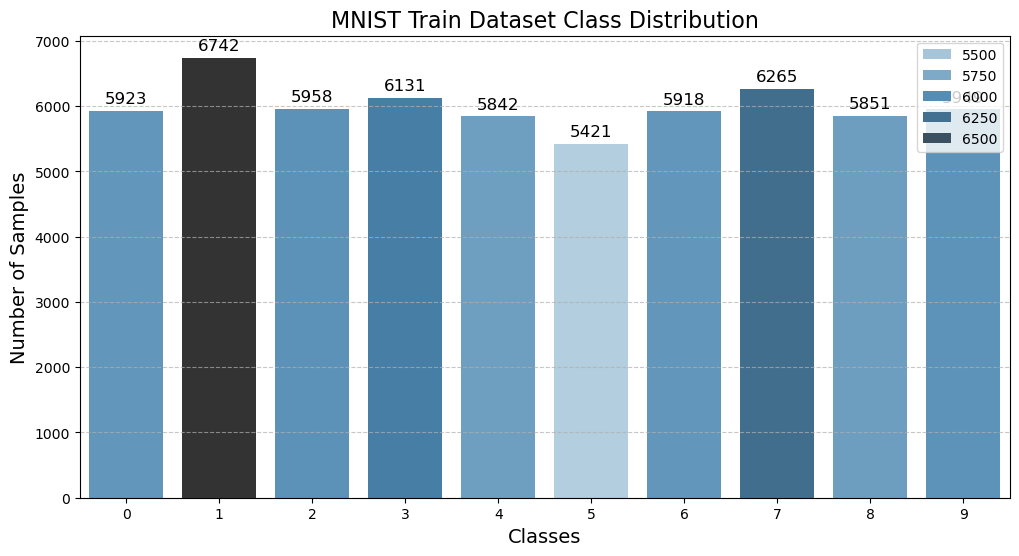
\includegraphics[width=0.4\textwidth, keepaspectratio]{mnist_train.png}
\end{figure}

\begin{figure}[h]
    \centering
    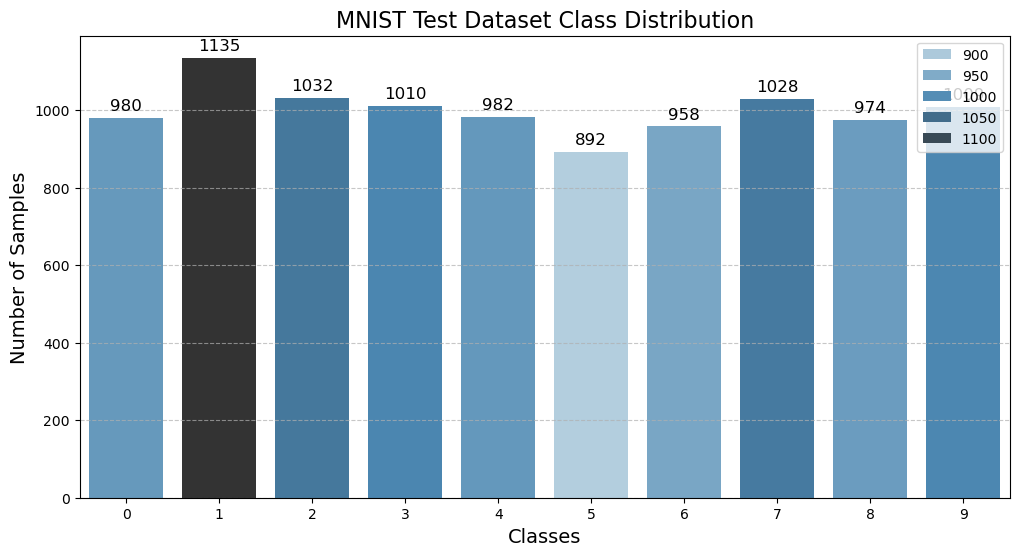
\includegraphics[width=0.4\textwidth, keepaspectratio]{mnist_test.png}
\end{figure}

Here is the visualization of all classes using bar plot to show the count of each class in the train and test dataset.

\vspace{0.5cm}
Now we extracted 1000 samples of each class 3, 4 and 7 from the training dataset and saved in the separate files for later use. Now 57000samples left in the training dataset that we saved in another file train\_rem.pkl. Now load the training dataset from train\_rem.pklfile also load the testing dataset. Following is the EDA of training and testing datasets.

Training data:
\begin{itemize}
    \item Total Samples: 57000
    \item Number of Classes: 10
    \item Classes: [0, 1, 2, 3, 4, 5, 6, 7, 8, 9]
  \item Train Data Shape: torch.Size([32, 1, 28, 28])
  \item Train Labels Shape: torch.Size([32])
\end{itemize}
\vspace{0.3cm}
Visualizing random samples of train dataset

\begin{figure}[h]
    \centering
    \includegraphics[width=0.4\textwidth, keepaspectratio]{train\_head.png}
\end{figure}


Testing Dataset:
\begin{itemize}
    \item Total Samples: 10000
    \item Number of Classes: 10
    \item Classes: [0, 1, 2, 3, 4, 5, 6, 7, 8, 9]
  \item Test Data Shape: torch.Size([32, 1, 28, 28])
  \item Train Test Labels Shape: torch.Size([32])
\end{itemize}
\vspace{0.3cm}
Visualizing random samples of test dataset

\begin{figure}[h]
    \centering
    \includegraphics[width=0.4\textwidth, keepaspectratio]{test\_head.png}
\end{figure}


\subsection{Enviornment Specifications}
It is necessary to stress that all factors of the experimental setting were chosen deliberately. The implementation was done in Python 3.12 and the PyTorch Lib 2.0.1 for purposes of model designing and training. Data cleaning and initial data exploration were done with NumPy and Pandas while the metric calculations were done with the use of scikit-learn 1.3.1. For data visualization, Matplotlib and Seaborn libraries were used because they provide easyness to understand plots and charts. The code execution was carried out from within Jupyter Notebook, which is operated from the Anaconda platform. Since, it was essential to maintain homogeneity and compartmentalization of all application dependent elements, a virtual environment was built out using pip and conda. The experiments were carried out on the CPU given the unavailability of a GPU, while computational threading was used to enhance concurrency.

The hardware specifications of the system used were as follows: A MacBook Pro using kernel release 24.1.0, architecture: x86\_64. The system was run with an OS of 2.8 GHz Quad-Core Intel Core i7 processor featuring 4 physical cores, 4 spares and thus 8 CPUs. For the computational needs in the experiments, it had 16 GB of 2133 MHz LPDDR3 RAM for sufficient resources.

\subsection{Methodology}
Let’s suppose you are a student and your professor assigned you a task to learn 30 topics till tomorrow, Will you be able to learn it? Yes, you can but your performance will be compromised. Now if you are asked to learn 10 topics in a day and total 30 topics in 3 days. Now your response will be much better as compared to first case. Here we used the same concept in our training. Instead of fine tuning our model on all three classes on a single run, we separately fine-tuned the model on each class. As a result, our model performed better when we separately fine-tuned model. 
We extracted 1000 samples of each class 3, 4 and 7 from the training dataset and saved in the separate files for later use. Now 57000 samples left in the training dataset that we saved in another file train\_rem.pkl. Now load the training dataset from train\_rem.pkl file also load the testing dataset. As we know train data contain 57000 samples and 10000 samples are in test data. After performing initial EDA, we define the Simple Neural Network (SimpleNN) model which we’ll use for training the model. Dataset is already splitted in training and testing. Then we use the Cross Entropy Loss function and Adam optimizer to minimize the loss function. Here is the mathematical representation of cross entropy loss.

\begin{equation}
H(p, q) = - \sum\_{x \in \mathcal{X}} p(x) \log q(x).
\end{equation}

We perform training on 57000 samples using 50 epochs with a batch size of 32 using SimpleNN model with 109386 parameters. We achieved 91.7\% accuracy on testing data when we test the dataset. Now after evaluation performance metrices we load those files that we have saved earlier. After performing its EDA, we further train these classes over the pretrained model step by step. First, we train class 3 samples on the pretrained model using 10 epochs and evaluate its performance. Similarly, we train and evaluate class 4 sample and class 7 samples reactively. Basically we are performing finetuning
After this we merge the all three classes samples together and then perform training using 10 epochs over the predefined model and then evaluate the performance.


\begin{figure}[h]
    \centering
    
\includegraphics[width=0.4\textwidth, keepaspectratio]{fig1.png}
    
\end{figure}


\section{Evaluation}
The proposed system MUSIC was trained on the MNIST digits dataset to 50 epochs. Thereupon, the datasets were partitioned into classes; some of the data, and the rest of the data was then utilized to train a pre-trained model. The classes which were extracted were 3, 4 and 7 chosen for further training both alone and in conjunction to obtain the end result. Training performance over the epochs portrayed a sign of improvement as illustrated by a reduction of training loss while the accuracy Continued to rise.  The accuracy for the final training set was 99.29\% while the accuracy for the test set was 91.78\% and the minimum value of test loss was 0.17. The outcomes of these metrics show that the model has a great potential on generalizing over the whole set in the first stage of the training.


\begin{figure}[h]
    \centering
    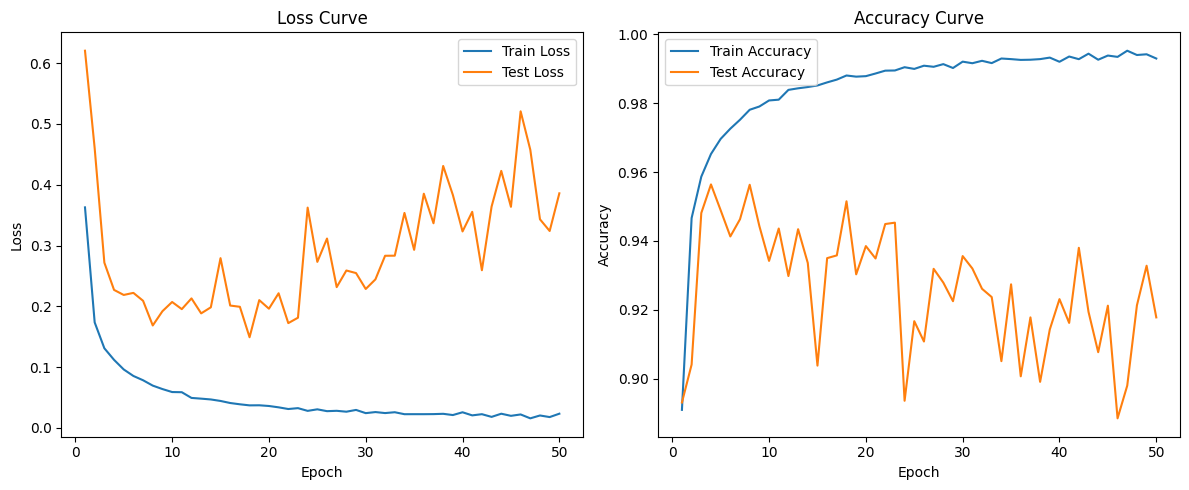
\includegraphics[width=0.3\textwidth, keepaspectratio]{predefined.png}
    
\end{figure}

To increase the performance of fine-tuning, the extracted classes were trained in separate from the pre-trained model for ten passes. In the fine-tuning process, performance for the individual classes was higher than the performance of the individual classes all summed up. In particular, the test accuracy obtained in class 3 was 83.61\%, while recall increased significantly. As for class 4, the achieved test accuracy is 86,62\%, while the precision and recall rates have been increased. Likewise, class 7 yielded a test accuracy of 87.53\% which corroborated that the proposed model is sensitive to individualistic class fine tuning. 


%``Fig.~\ref{fig}'', even at the beginning of a sentence.

On the other hand, when the classes were introduced into a unified dataset for jointly fine-tuning the test accuracy came down to 70.03\%. This decline implies that there might be some issues related to dataset biases or of generalization performance when using merged class datasets.

The metrics of classification also show us the efficiency of the entire model and what aspects could be improved. For class 1, the highest precision of 0.99 was achieved, whereas for class 0 the highest recall of 0.98 was obtained with the average F1-score of 0.92 of the baseline model. By looking at the confusion matrix it was evident that the proposed model was more accurate when fine-tuned on singular classes over the merged data set. They also reported problems when interpreting numbers that are visually similar: 3 and 8 for example. The structure of the confusion matrix helped to identify additional information about model performance for individual or merged classes and support the idea of fine-tuning for certain classes.


\begin{figure}[h]
    \centering
    \includegraphics[width=0.3\textwidth, keepaspectratio]{class\_7\_conf.png}
    
\end{figure}
%``Fig.~\ref{fig}'', even at the beginning of a sentence.

\begin{table}[htbp]
\caption{Performance Evaluation Table}
\begin{center}
\begin{tabular}{|c|c|c|}
\hline
\textbf{Data} & \textbf{Accuracy (\%)} & \textbf{Loss} \\ 
\hline
Pre-trained model & 92 & 0.38 \\ 
\hline
Fine-tuned on combined tasks & 70 & 2.1 \\ 
\hline
Fine-tuned on individual tasks & 88 & 0.60 \\ 
\hline
\end{tabular}
\label{tab:performance}
\end{center}
\end{table}



\section{Conclusion}
In this paper we introduced the best practice to fine-tune the models. For Images dataset the model performed well following out technique. Fine-tune the model individually on each task results in better accuracy as compared to fine-tune on combined tasks. This technique is simple but has a huge impact in terms of transfer learning. We will further test it on other datasets for generalization and then move to next step which is to edit models through task arithmetic (Addition or Subtraction).


\begin{thebibliography}{00}
\bibitem{paper-1} Gabriel Ilharco, Marco Tulio Ribeiro, Mitchell Wortsman, Suchin Gururangan, Ludwig Schmidt, Hannaneh Hajishirzi, Ali Farhadi, EDITING MODELS WITH TASK ARITHMETIC, 2024.
\bibitem{paper-2} Rishabh Bhardwaj, Do Duc Anh, and Soujanya Poria, Language Models are Homer Simpson! Safety Re-Alignment of Fine-tuned Language Models through Task Arithmetic, 2024.
\bibitem{paper-3} Guillermo Ortiz-Jimenez and Alessandro Favero,Task Arithmetic in the Tangent Space:Improved Editing of Pre-Trained Models, 2024.

\end{thebibliography}


\end{document}
